\documentclass[../main.tex]{subfiles}

\begin{document}
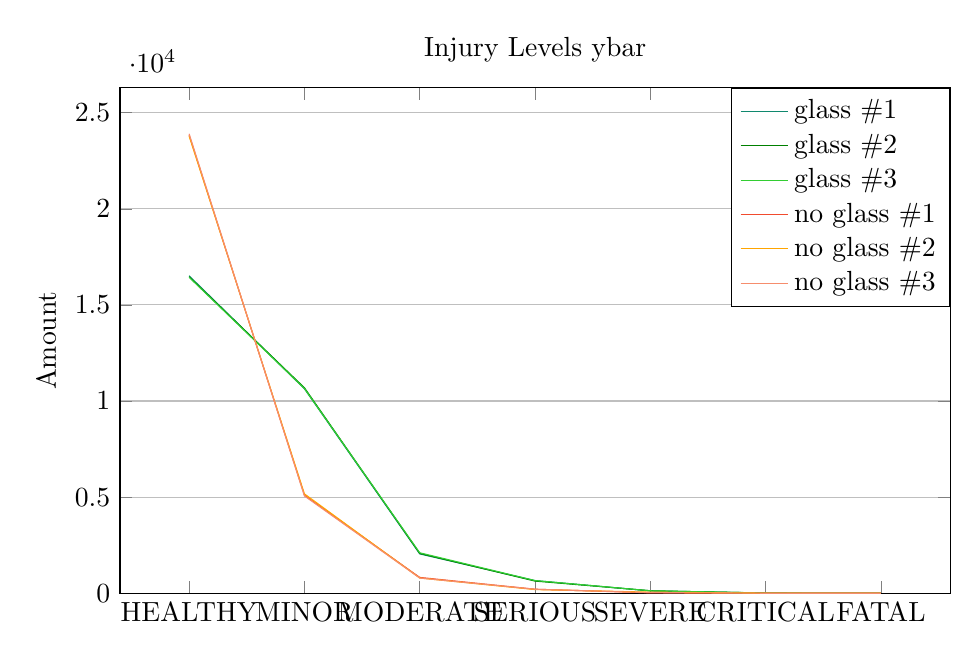
\begin{tikzpicture}
\begin{axis}[
title={Injury Levels}
ybar, % style of the histogram: clustered columns
width=\textwidth, % width of the plot
height=8cm, % height of the plot
ylabel={Amount}, % label for the y-axis
symbolic x coords={HEALTHY,MINOR,MODERATE,SERIOUS,SEVERE,CRITICAL,FATAL}, % labels for the x-ticks
xtick=data, % position the x-ticks at the data points
ymin=0, % minimum value of the y-axis
legend style={at={(1,1)}, anchor=north east}, % position of the legend
legend cell align=left, % alignment of the legend cells
ymajorgrids=true, % display major grids
bar width=0.25cm % width of the bars
]
\addplot[color=PineGreen] coordinates{(HEALTHY,16515)(MINOR,10639)(MODERATE,2047)(SERIOUS,660)(SEVERE,124)(CRITICAL,13)(FATAL,2)
}; % plot of the first histogram
\addplot[color=Green] coordinates{(HEALTHY,16461)(MINOR,10690)(MODERATE,2074)(SERIOUS,634)(SEVERE,131)(CRITICAL,9)(FATAL,1)
}; % plot of the second histogram
\addplot[color=LimeGreen] coordinates{(HEALTHY,16438)(MINOR,10650)(MODERATE,2106)(SERIOUS,660)(SEVERE,129)(CRITICAL,15)(FATAL,2)
}; % plot of the third histogram
\addplot[color=RedOrange] coordinates{(HEALTHY,23840)(MINOR,5101)(MODERATE,824)(SERIOUS,211)(SEVERE,23)(CRITICAL,1)(FATAL,0)
}; % plot of the fourth histogram
\addplot[color=Orange] coordinates{(HEALTHY,23781)(MINOR,5170)(MODERATE,793)(SERIOUS,192)(SEVERE,58)(CRITICAL,6)(FATAL,0)
}; % plot of the fifth histogram
\addplot[color=Melon] coordinates{(HEALTHY,23902)(MINOR,5062)(MODERATE,791)(SERIOUS,210)(SEVERE,33)(CRITICAL,2)(FATAL,0)
}; % plot of the first histogram
\legend{glass \#1,  glass \#2, glass \#3, no glass \#1,  no glass \#2, no glass \#3,} % legend of the plot
\end{axis}
\end{tikzpicture}
\end{document}